%% GENERATED by scripts/make_figure1.py -- edit the generator, not this file.
\documentclass[border=6pt]{standalone}
\usepackage{tikz}
\usetikzlibrary{arrows.meta}
\usepackage{sansmath}
\renewcommand{\familydefault}{\sfdefault}
\sansmath
\definecolor{ink}{HTML}{1B2430}
\definecolor{inkdim}{HTML}{5D7185}
\definecolor{gridc}{HTML}{C9D3DE}
\definecolor{sph}{HTML}{D9DEE4}
\definecolor{sub}{HTML}{C8CED6}
\definecolor{shellc}{HTML}{EEF1F5}
\definecolor{uhi}{HTML}{1D3A7A}
\definecolor{ulo}{HTML}{F5DFA0}
\definecolor{spA}{HTML}{1D3A7A}
\definecolor{spB}{HTML}{A4C639}
\definecolor{spAB}{HTML}{2BB3A3}
\tikzset{
  gridl/.style={draw=gridc, line width=0.5pt},
  gridb/.style={draw=gridc!70!ink, line width=0.6pt},
  shell/.style={fill=shellc},
  op/.style={-{Stealth[length=7pt,width=5pt]}, line width=1.4pt, ink},
  mv/.style={-{Stealth[length=4pt,width=3.5pt]}, line width=0.9pt, ink},
  gen/.style={-{Stealth[length=5pt]}, line width=0.9pt, inkdim},
  lbl/.style={font=\small, ink},
  reads/.style={-{Stealth[length=5pt]}, line width=0.9pt, inkdim, dashed},
}
\newcommand{\num}[1]{\tikz[baseline=(n.base)]\node[draw=ink, circle, line width=0.6pt, inner sep=0.8pt, font=\scriptsize](n){#1};}
\begin{document}
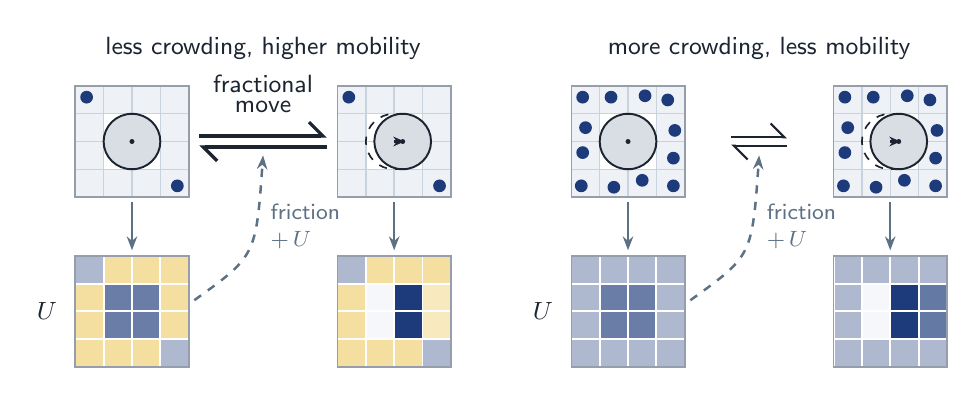
\begin{tikzpicture}[x=0.9cm, y=0.88cm]
\fill[shell] (2.100,-2.450) rectangle ++(0.400,0.400);
\fill[shell] (2.100,-2.050) rectangle ++(0.400,0.400);
\fill[shell] (2.100,-1.650) rectangle ++(0.400,0.400);
\fill[shell] (2.100,-1.250) rectangle ++(0.400,0.400);
\fill[shell] (2.500,-2.450) rectangle ++(0.400,0.400);
\fill[shell] (2.500,-1.250) rectangle ++(0.400,0.400);
\fill[shell] (2.900,-2.450) rectangle ++(0.400,0.400);
\fill[shell] (2.900,-1.250) rectangle ++(0.400,0.400);
\fill[shell] (3.300,-2.450) rectangle ++(0.400,0.400);
\fill[shell] (3.300,-2.050) rectangle ++(0.400,0.400);
\fill[shell] (3.300,-1.650) rectangle ++(0.400,0.400);
\fill[shell] (3.300,-1.250) rectangle ++(0.400,0.400);
\draw[gridl, shift={(2.100,-2.450)}] (0,0) grid[step=0.400] (1.600,1.600);
\draw[gridb] (2.100,-2.450) rectangle (3.700,-0.850);
\fill[sph, draw=ink, line width=0.7pt] (2.900,-1.650) circle (0.400);
\fill[ink] (2.900,-1.650) circle (0.9pt);
\fill[spA] (2.260,-1.010) circle (2.3pt);
\fill[spA] (3.540,-2.290) circle (2.3pt);
\draw[gen] (2.900,-2.530) -- (2.900,-3.220);
\fill[shell] (5.800,-2.450) rectangle ++(0.400,0.400);
\fill[shell] (5.800,-2.050) rectangle ++(0.400,0.400);
\fill[shell] (5.800,-1.650) rectangle ++(0.400,0.400);
\fill[shell] (5.800,-1.250) rectangle ++(0.400,0.400);
\fill[shell] (6.200,-2.450) rectangle ++(0.400,0.400);
\fill[shell] (6.200,-1.250) rectangle ++(0.400,0.400);
\fill[shell] (6.600,-2.450) rectangle ++(0.400,0.400);
\fill[shell] (6.600,-1.250) rectangle ++(0.400,0.400);
\fill[shell] (7.000,-2.450) rectangle ++(0.400,0.400);
\fill[shell] (7.000,-2.050) rectangle ++(0.400,0.400);
\fill[shell] (7.000,-1.650) rectangle ++(0.400,0.400);
\fill[shell] (7.000,-1.250) rectangle ++(0.400,0.400);
\draw[gridl, shift={(5.800,-2.450)}] (0,0) grid[step=0.400] (1.600,1.600);
\draw[gridb] (5.800,-2.450) rectangle (7.400,-0.850);
\draw[ink, dashed, line width=0.6pt] (6.600,-1.650) circle (0.400);
\fill[sph, draw=ink, line width=0.7pt] (6.720,-1.650) circle (0.400);
\fill[ink] (6.720,-1.650) circle (0.9pt);
\draw[mv] (6.600,-1.650) -- (6.744,-1.650);
\fill[spA] (5.960,-1.010) circle (2.3pt);
\fill[spA] (7.240,-2.290) circle (2.3pt);
\draw[gen] (6.600,-2.530) -- (6.600,-3.220);
\draw[-{Straight Barb[left,length=5pt]}, line width=1.2pt, ink] (3.850,-1.570) -- (5.650,-1.570);
\draw[-{Straight Barb[left,length=5pt]}, line width=1.2pt, ink] (5.650,-1.730) -- (3.850,-1.730);
\node[lbl, above=7pt] at (4.750,-1.650) {\shortstack{fractional\\move}};
\draw[reads] (3.780,-3.940) .. controls (4.650,-3.300) .. (4.750,-1.850);
\node[anchor=west, align=left, font=\footnotesize, inkdim, inner sep=0pt] at (4.850,-2.875) {friction\\$+\,U$};
\node[lbl, anchor=center] at (4.750,-0.300) {less crowding, higher mobility};
\node[lbl, anchor=east] at (1.980,-4.100) {$U$};
\fill[shell] (9.100,-2.450) rectangle ++(0.400,0.400);
\fill[shell] (9.100,-2.050) rectangle ++(0.400,0.400);
\fill[shell] (9.100,-1.650) rectangle ++(0.400,0.400);
\fill[shell] (9.100,-1.250) rectangle ++(0.400,0.400);
\fill[shell] (9.500,-2.450) rectangle ++(0.400,0.400);
\fill[shell] (9.500,-1.250) rectangle ++(0.400,0.400);
\fill[shell] (9.900,-2.450) rectangle ++(0.400,0.400);
\fill[shell] (9.900,-1.250) rectangle ++(0.400,0.400);
\fill[shell] (10.300,-2.450) rectangle ++(0.400,0.400);
\fill[shell] (10.300,-2.050) rectangle ++(0.400,0.400);
\fill[shell] (10.300,-1.650) rectangle ++(0.400,0.400);
\fill[shell] (10.300,-1.250) rectangle ++(0.400,0.400);
\draw[gridl, shift={(9.100,-2.450)}] (0,0) grid[step=0.400] (1.600,1.600);
\draw[gridb] (9.100,-2.450) rectangle (10.700,-0.850);
\fill[sph, draw=ink, line width=0.7pt] (9.900,-1.650) circle (0.400);
\fill[ink] (9.900,-1.650) circle (0.9pt);
\fill[spA] (9.260,-1.010) circle (2.3pt);
\fill[spA] (10.540,-2.290) circle (2.3pt);
\fill[spA] (9.240,-2.290) circle (2.3pt);
\fill[spA] (9.260,-1.810) circle (2.3pt);
\fill[spA] (9.700,-2.310) circle (2.3pt);
\fill[spA] (10.140,-0.990) circle (2.3pt);
\fill[spA] (10.560,-1.490) circle (2.3pt);
\fill[spA] (10.540,-1.890) circle (2.3pt);
\fill[spA] (9.660,-1.010) circle (2.3pt);
\fill[spA] (9.300,-1.450) circle (2.3pt);
\fill[spA] (10.100,-2.210) circle (2.3pt);
\fill[spA] (10.460,-1.050) circle (2.3pt);
\draw[gen] (9.900,-2.530) -- (9.900,-3.220);
\fill[shell] (12.800,-2.450) rectangle ++(0.400,0.400);
\fill[shell] (12.800,-2.050) rectangle ++(0.400,0.400);
\fill[shell] (12.800,-1.650) rectangle ++(0.400,0.400);
\fill[shell] (12.800,-1.250) rectangle ++(0.400,0.400);
\fill[shell] (13.200,-2.450) rectangle ++(0.400,0.400);
\fill[shell] (13.200,-1.250) rectangle ++(0.400,0.400);
\fill[shell] (13.600,-2.450) rectangle ++(0.400,0.400);
\fill[shell] (13.600,-1.250) rectangle ++(0.400,0.400);
\fill[shell] (14.000,-2.450) rectangle ++(0.400,0.400);
\fill[shell] (14.000,-2.050) rectangle ++(0.400,0.400);
\fill[shell] (14.000,-1.650) rectangle ++(0.400,0.400);
\fill[shell] (14.000,-1.250) rectangle ++(0.400,0.400);
\draw[gridl, shift={(12.800,-2.450)}] (0,0) grid[step=0.400] (1.600,1.600);
\draw[gridb] (12.800,-2.450) rectangle (14.400,-0.850);
\draw[ink, dashed, line width=0.6pt] (13.600,-1.650) circle (0.400);
\fill[sph, draw=ink, line width=0.7pt] (13.720,-1.650) circle (0.400);
\fill[ink] (13.720,-1.650) circle (0.9pt);
\draw[mv] (13.600,-1.650) -- (13.744,-1.650);
\fill[spA] (12.960,-1.010) circle (2.3pt);
\fill[spA] (14.240,-2.290) circle (2.3pt);
\fill[spA] (12.940,-2.290) circle (2.3pt);
\fill[spA] (12.960,-1.810) circle (2.3pt);
\fill[spA] (13.400,-2.310) circle (2.3pt);
\fill[spA] (13.840,-0.990) circle (2.3pt);
\fill[spA] (14.260,-1.490) circle (2.3pt);
\fill[spA] (14.240,-1.890) circle (2.3pt);
\fill[spA] (13.360,-1.010) circle (2.3pt);
\fill[spA] (13.000,-1.450) circle (2.3pt);
\fill[spA] (13.800,-2.210) circle (2.3pt);
\fill[spA] (14.160,-1.050) circle (2.3pt);
\draw[gen] (13.600,-2.530) -- (13.600,-3.220);
\draw[-{Straight Barb[left,length=5pt]}, line width=0.8pt, ink] (11.354,-1.590) -- (12.146,-1.590);
\draw[-{Straight Barb[left,length=5pt]}, line width=0.8pt, ink] (12.146,-1.710) -- (11.354,-1.710);
\draw[reads] (10.780,-3.940) .. controls (11.650,-3.300) .. (11.750,-1.850);
\node[anchor=west, align=left, font=\footnotesize, inkdim, inner sep=0pt] at (11.850,-2.875) {friction\\$+\,U$};
\node[lbl, anchor=center] at (11.750,-0.300) {more crowding, less mobility};
\node[lbl, anchor=east] at (8.980,-4.100) {$U$};
\fill[ulo!100!white] (2.100,-4.900) rectangle ++(0.400,0.400);
\fill[ulo!100!white] (2.500,-4.900) rectangle ++(0.400,0.400);
\fill[ulo!100!white] (2.900,-4.900) rectangle ++(0.400,0.400);
\fill[uhi!36!white] (3.300,-4.900) rectangle ++(0.400,0.400);
\fill[ulo!100!white] (2.100,-4.500) rectangle ++(0.400,0.400);
\fill[uhi!66!white] (2.500,-4.500) rectangle ++(0.400,0.400);
\fill[uhi!66!white] (2.900,-4.500) rectangle ++(0.400,0.400);
\fill[ulo!100!white] (3.300,-4.500) rectangle ++(0.400,0.400);
\fill[ulo!100!white] (2.100,-4.100) rectangle ++(0.400,0.400);
\fill[uhi!66!white] (2.500,-4.100) rectangle ++(0.400,0.400);
\fill[uhi!66!white] (2.900,-4.100) rectangle ++(0.400,0.400);
\fill[ulo!100!white] (3.300,-4.100) rectangle ++(0.400,0.400);
\fill[uhi!36!white] (2.100,-3.700) rectangle ++(0.400,0.400);
\fill[ulo!100!white] (2.500,-3.700) rectangle ++(0.400,0.400);
\fill[ulo!100!white] (2.900,-3.700) rectangle ++(0.400,0.400);
\fill[ulo!100!white] (3.300,-3.700) rectangle ++(0.400,0.400);
\draw[white, line width=0.7pt, shift={(2.100,-4.900)}] (0,0) grid[step=0.400] (1.600,1.600);
\draw[gridb] (2.100,-4.900) rectangle (3.700,-3.300);
\fill[ulo!100!white] (5.800,-4.900) rectangle ++(0.400,0.400);
\fill[ulo!100!white] (6.200,-4.900) rectangle ++(0.400,0.400);
\fill[ulo!100!white] (6.600,-4.900) rectangle ++(0.400,0.400);
\fill[uhi!36!white] (7.000,-4.900) rectangle ++(0.400,0.400);
\fill[ulo!100!white] (5.800,-4.500) rectangle ++(0.400,0.400);
\fill[uhi!4!white] (6.200,-4.500) rectangle ++(0.400,0.400);
\fill[uhi!100!white] (6.600,-4.500) rectangle ++(0.400,0.400);
\fill[ulo!68!white] (7.000,-4.500) rectangle ++(0.400,0.400);
\fill[ulo!100!white] (5.800,-4.100) rectangle ++(0.400,0.400);
\fill[uhi!4!white] (6.200,-4.100) rectangle ++(0.400,0.400);
\fill[uhi!100!white] (6.600,-4.100) rectangle ++(0.400,0.400);
\fill[ulo!68!white] (7.000,-4.100) rectangle ++(0.400,0.400);
\fill[uhi!36!white] (5.800,-3.700) rectangle ++(0.400,0.400);
\fill[ulo!100!white] (6.200,-3.700) rectangle ++(0.400,0.400);
\fill[ulo!100!white] (6.600,-3.700) rectangle ++(0.400,0.400);
\fill[ulo!100!white] (7.000,-3.700) rectangle ++(0.400,0.400);
\draw[white, line width=0.7pt, shift={(5.800,-4.900)}] (0,0) grid[step=0.400] (1.600,1.600);
\draw[gridb] (5.800,-4.900) rectangle (7.400,-3.300);
\fill[uhi!36!white] (9.100,-4.900) rectangle ++(0.400,0.400);
\fill[uhi!36!white] (9.500,-4.900) rectangle ++(0.400,0.400);
\fill[uhi!36!white] (9.900,-4.900) rectangle ++(0.400,0.400);
\fill[uhi!36!white] (10.300,-4.900) rectangle ++(0.400,0.400);
\fill[uhi!36!white] (9.100,-4.500) rectangle ++(0.400,0.400);
\fill[uhi!66!white] (9.500,-4.500) rectangle ++(0.400,0.400);
\fill[uhi!66!white] (9.900,-4.500) rectangle ++(0.400,0.400);
\fill[uhi!36!white] (10.300,-4.500) rectangle ++(0.400,0.400);
\fill[uhi!36!white] (9.100,-4.100) rectangle ++(0.400,0.400);
\fill[uhi!66!white] (9.500,-4.100) rectangle ++(0.400,0.400);
\fill[uhi!66!white] (9.900,-4.100) rectangle ++(0.400,0.400);
\fill[uhi!36!white] (10.300,-4.100) rectangle ++(0.400,0.400);
\fill[uhi!36!white] (9.100,-3.700) rectangle ++(0.400,0.400);
\fill[uhi!36!white] (9.500,-3.700) rectangle ++(0.400,0.400);
\fill[uhi!36!white] (9.900,-3.700) rectangle ++(0.400,0.400);
\fill[uhi!36!white] (10.300,-3.700) rectangle ++(0.400,0.400);
\draw[white, line width=0.7pt, shift={(9.100,-4.900)}] (0,0) grid[step=0.400] (1.600,1.600);
\draw[gridb] (9.100,-4.900) rectangle (10.700,-3.300);
\fill[uhi!36!white] (12.800,-4.900) rectangle ++(0.400,0.400);
\fill[uhi!36!white] (13.200,-4.900) rectangle ++(0.400,0.400);
\fill[uhi!36!white] (13.600,-4.900) rectangle ++(0.400,0.400);
\fill[uhi!36!white] (14.000,-4.900) rectangle ++(0.400,0.400);
\fill[uhi!36!white] (12.800,-4.500) rectangle ++(0.400,0.400);
\fill[uhi!4!white] (13.200,-4.500) rectangle ++(0.400,0.400);
\fill[uhi!100!white] (13.600,-4.500) rectangle ++(0.400,0.400);
\fill[uhi!68!white] (14.000,-4.500) rectangle ++(0.400,0.400);
\fill[uhi!36!white] (12.800,-4.100) rectangle ++(0.400,0.400);
\fill[uhi!4!white] (13.200,-4.100) rectangle ++(0.400,0.400);
\fill[uhi!100!white] (13.600,-4.100) rectangle ++(0.400,0.400);
\fill[uhi!68!white] (14.000,-4.100) rectangle ++(0.400,0.400);
\fill[uhi!36!white] (12.800,-3.700) rectangle ++(0.400,0.400);
\fill[uhi!36!white] (13.200,-3.700) rectangle ++(0.400,0.400);
\fill[uhi!36!white] (13.600,-3.700) rectangle ++(0.400,0.400);
\fill[uhi!36!white] (14.000,-3.700) rectangle ++(0.400,0.400);
\draw[white, line width=0.7pt, shift={(12.800,-4.900)}] (0,0) grid[step=0.400] (1.600,1.600);
\draw[gridb] (12.800,-4.900) rectangle (14.400,-3.300);
\end{tikzpicture}
\end{document}
